\chapter{Trusted Execution Environments} \label{tees}

Trusted Execution Environment (TEE) is a secure environment of a computing device that is isolated from the rest of the system and has its own isolated memory and processing capabilities, preserving confidentiality and integrity. Trusted Execution Environments are not precisely defined, but solutions called TEE's usually have in common that they try to protect the data-in-use, as the more conventional encryption solutions try to protect data-at-rest and data-in-transit. This chapter partly answers to the \ref{rq1}.

Trusted Execution Environments are usually implemented by secure architecture that makes use of hardware features of CPU. TEE's provide a confidential and isolated processing environment, usually backed by hardware-assisted memory encryption.

The idea of TEE's is to provide an isolated environment that is secured from investigation by the rest of the system, allowing development of applications that require high security. For example, TEE's can be used to build systems that allow securing intellectual property, processing of sensitive personal information securely, Digital Rights Management (DRM), secure financial services etc.\cite{teeieee}

As the solution proposed by this thesis is based on Intel's Trusted Execution Environment called Intel Software Guard Extensions (Intel SGX), we focus mainly on that technology, but giving high-level introduction to other TEE platforms.

\section{Use Cases}\label{usecases}

\subsection{Protecting Intellectual Property}\label{protecting1}


With TEE's the decryption and processing of the data can happen completely in a secure environment without the possibility to investigate the data in clear form. This usually requires that the TEE establishes a secure connection for authentication and encryption key exchange outside the environment.

For example, machine learning models can be bundled with application encrypted. The application then decrypts the models only when needed, inside the Trusted Execution Environment.

\subsubsection{Digital Rights Management (DRM)}\label{protecting11}

TEE's provide means for advanced Digital Rights Management. For example, streaming services can protect its content by encrypting the stream data. Encrypted stream data can then be decrypted by the isolated TEE, thus disallowing the customer to copy the content.

\subsection{Protecting Sensitive Personal Information}\label{protecting2}

Sensitive information can be stored encrypted and only decrypted for processing inside the Trusted Execution Environment. This is the case, especially when sensitive information needs to be stored and processed in an untrusted cloud environment.

\subsection{Financial Services}\label{protecting3}

Financial services often have a high security standards. TEE's can help financial services to fulfill these standards by allowing storing and using keys or tokens needed for transactions in an encrypted and isolated environment.

Especially, commerce platforms on mobile devices including Near-Field Communication (NFC) to authorization can benefit from Trusted Execution Environments.

\subsection{Biometric Authentication}\label{protecting4}

The problem with biometric authentication is that the sample of a correct biometric authentication method has to be stored somewhere that then can be compared to input. For example, in a case of fingerprint authentication, the sample of an authorized person's fingerprint needs to be stored in some form. When the sample is stored unprotected, it is possible to retrieve it and use it for authentication.

With TEE's the sample can be stored encrypted and the comparing process can then happen completely in the isolated environment, where the sample is decrypted, thus disallowing any investigation of the sample by the outside world.

\section{Intel Software Guard Extensions (Intel SGX)}\label{sgx}

Intel introduced new security-related instruction codes called Security Guard Extensions (SGX) in 2015 part of the sixth generation Intel Core processor family release. At the time of writing this thesis (2023), Intel has dropped support for SGX in consumer CPU model Intel Core, but continues development on the enterprise Intel Xeon series of processors.

Software Guard Extensions allow user- or operating system -level code to create hardware-backed secure and isolated processing environments, called Enclaves. Enclaves are in a specific isolated and encrypted part of the memory and content is decrypted on the fly inside the CPU when processing.

Code inside the enclave cannot be examined by the rest of the system by any code that is running with higher privileges, not even by computer firmware or hypervisors in a virtual environment.

In the Intel SGX application, the application code is divided into trusted and untrusted parts. The untrusted part handles the creation of the enclave and communication with the rest of the system. The trusted part runs inside the enclave. Usually, most of the application code is in the untrusted part, as it is recommended to operate inside the enclave only when it is really necessary, due to the limited memory of the enclave.\cite{mit}

Intel SGX has some vulnerabilities, most of them based on the side-channel attack.\cite{sgxfail}

\subsection{Remote Attestation}\label{remoteattestation}

Remote attestation is an Intel SGX feature that enables trust between a remote server and the application running in the Intel SGX enclave. The remote server can verify that the application is, in fact, running in the fully working SGX enclave and all the latest security patches are applied.

The main use case of remote attestation is to verify that it is safe to open up the secure channel between the remote server and the application running in the enclave. After the remote attestation is complete, information can be exchanged safely through the secure channel.

Intel provides two different methods for remote attestation. Enhanced Privacy ID (Intel EPID) based attestation method can be used on older Intel SGX capable processors that do not support Flexible Launch Control. This attestation method requires usage of Intel's attestation service.

Elliptic Curve Digital Signature Algorithm (ECDSA) Attestation is the second of the attestation methods. This method requires newer processor models that support Flexible Launch Control. On the other hand, the attestation service can be self-hosted.

\subsection{Using Intel SGX on Linux}\label{usingsgxonlinux}

Running Intel SGX applications on Linux requires two software parts to be installed: Intel SGX driver and Intel SGX Platform Software (PSW). 
To be able to build Intel SGX applications, also the Intel SGX Software Development Kit (SDK) needs to be installed. Of course, the Intel SGX support needs to be enabled on the hardware level (BIOS/UEFI) too. Intel provides repositories for software required for the supported Linux distributions.

Currently, Intel supports the next Linux distributions: Red Hat Enterprise Linux, CentOS Server, Ubuntu Server, SUSE Linux Enterprise Server, Anolis OS, Debian.

The Linux kernel supports Intel SGX natively from kernel version 5.11, but only processor models with Flexible Launch Control support. If the processor does not support Flexible Launch Control, the Out-of-Tree (OOT) driver and kernel version lower than 5.11 must be used.

To check that the Intel SGX support is enabled, \textit{cpuid} utility could be used. Example lines from \textit{cpuid} output showing Intel SGX support in Listing \ref{alg:cpuid}.

\begin{algorithm}
\begin{minted}{text}
  Software Guard Extensions (SGX) capability (0x12/0):
      SGX1 supported                           = true
      SGX2 supported                           = false
\end{minted}
\caption{Example cpuid output for discovering Intel SGX support.\label{alg:cpuid}}
\end{algorithm}

Intel has provided very detailed installation instructions for all the software parts needed for different platforms and processor models.\cite{sgxinstall} The Intel SGX SDK has a directory \textit{SampleCode} which contains multiple C++ application and build configuration examples.

\subsection{Limitations}\label{limitations}

The additional security provided by Intel SGX does not come free of limitations. The most obvious limitation is that the hardware must be chosen from Intel processors that have Intel SGX support. Running applications inside an Intel SGX enclave has limited performance. From the perspective of a processor-heavy machine learning calculations, the limited performance might be an issue. The performance degradation is discussed in detail in the Section \ref{performance}.

Another limitation is that the enclave size is limited by the maximum amount of memory that an enclave can allocate. The maximum memory amount that can be allocated is determined mainly by the Enclave Page Cache (EPC) size that is usually between 64 MB and 256 MB and depends on the processor model and firmware. On Linux, the EPC size limit can be bypassed by EPC swapping, but that adds additional performance overhead. \cite{graminedocs}

On the modern Intel Xeon server processors, starting with Ice Lake models, the EPC size can be up to 1 TB. With the 1 TB limit, the size of an enclave does not be an issue in most cases.

The EPC size can be discovered by Gramine\cite{gramine} utility \textit{is-sgx-available}. Example output can be seen in Listing \ref{alg:issgx}. The example output reports the EPC size to be 5d80000 bytes in hexadecimal, which is 98041856 bytes (98 MB) in decimal. 

The limitations of the development process of an Intel SGX application must also be considered. Intel SGX applications must be written in C or C++ and they must follow specific structure. Intel SGX does not allow dynamic linking, so libraries must be statically linked to the application. Many popular machine learning libraries for C++ do not offer a statically linked version of the library.\cite{sgxdev}

The development process restrictions can be eased with frameworks like Gramine\cite{gramine} which can wrap, for example, applications written in Python in Intel SGX compatible application. Gramine is discussed in more detail in the next section.

\begin{algorithm}
\begin{minted}{text}
...
Max enclave size (32-bit): 0x80000000
Max enclave size (64-bit): 0x1000000000
EPC size: 0x5d80000
SGX driver loaded: true
...
\end{minted}
\caption{Example is-sgx-available output for discovering EPC size.\label{alg:issgx}}
\end{algorithm}

\subsection{Gramine LibOS}\label{gramine}

Gramine is a lightweight Library Operating System (LibOS) which allows single applications to be run isolated with a minimal operating system. Gramine was first developed in OSCAR LAB at Stony Brook University, but many contributors joined the development process, including Intel Research Lab, which contributed to the Intel SGX support. 

Library operating system can be compared to running a full operating system inside a virtual machine, but much more lightweight and minimalistic approach.

Gramine allows applications to be run inside the Intel SGX enclave without the need to port them to Intel SGX C or C++ applications. Even applications written in interpreted languages, like Python, can be run inside enclave. Gramine enables this by wrapping the application code with interpreter and needed libraries inside a Gramine application, which can be then run inside the Intel SGX enclave.\cite{graminedocs}

The Gramine LibOS itself adds a memory cost just of 5 to 15 MB, but when running Gramine application inside Intel SGX enclave, other performance implications appear. In the paper\cite{graminesgxwp} by the Gramine team from 2017, the performance effects of running simple operations inside the Intel SGX enclave were discussed. Based on the measurements that Gramine team has conducted, running simple operations inside an enclave were approximately 100\% slower than locally, as can be seen in Figure \ref{img:graminebenchmark}. The more memory intensive the operation was, the more overhead it adds.

\begin{figure}
\centering 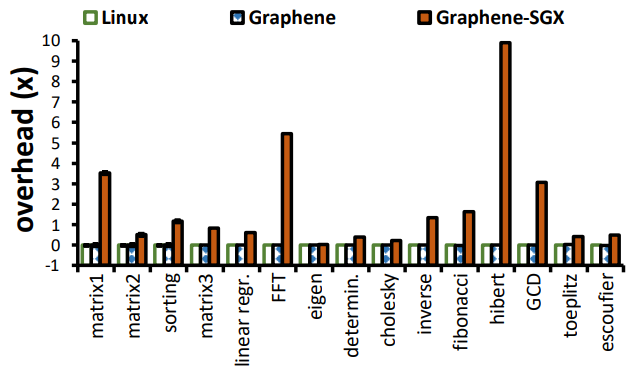
\includegraphics[width=0.7\textwidth]{img/graminebenchmark}
\caption{Performance overhead of Graphene-SGX, presented in \textit{Graphene-SGX: A Practical Library {OS} for Unmodified Applications on SGX}}
\label{img:graminebenchmark} 
\end{figure}

Gramine applications are configured in a special manifest file which uses TOML syntax. Configurable values include application entry point, enclave settings, remote attestation settings and trusted files. A part of a manifest file from the implementation that is provided as a part of this thesis can be seen in Listing \ref{alg:graminetoml}.

\begin{algorithm}
\begin{minted}{toml}
sgx.trusted_files = [
    ...
    "file:trusted.py",
    "file:ca.crt",
    "file:model_encrypted",
    "file:cars.csv",
]
\end{minted}
\caption{Part of Gramine application manifest file defining trusted files\label{alg:graminetoml}}
\end{algorithm}

Installation and usage of Gramine is discussed in the Chapter \ref{solution}. In the Section \ref{performance}, it can be seen how measurements conducted in this thesis aligns with the measurements conducted by Gramine team.

\section{AMD Secure Encrypted Virtualization (SEV)} \label{sev}

AMD's Secure Encrypted Virtualization (SEV) is a hardware-backed Trusted Execution Environment platform that allows an encryption of a virtual machine memory. AMD SEV is supported on AMD EPYC server processors. AMD SEV requires usage of the Linux built-in hypervisor Kernel-based Virtual Machine (KVM).

AMD SEV has no need for code changes to the application, as the whole memory used by the virtual machine is encrypted. There are also no memory limits other than physical memory. On the other hand, security features are limited compared to the Intel SGX.\cite{suse}

\section{ARM TrustZone} \label{trustzone}

ARM TrustZone is the oldest and the most used Trusted Execution Environment platform mentioned in this thesis. AMD TrustZone is a hardware-backed TEE supported on ARM Cortex-A and ARM Cortex-M microcontrollers, first introduced in 2004. There are some differing infrastructure details between the implementation of the Cortex-A and Cortex-M microcontroller families. The main usage platform is mobile devices, and some of the mobile device manufactures use ARM TrustZone comprehensively.\cite{trustzone}

\section{Cloud Provider's Solutions} \label{cloudprovider}

Amazon Web Services (AWS), Google Cloud Platforms (GCP) and Microsoft Azure all offer Trusted Execution Environment implementation on their cloud computing platforms. They are rather novel technologies, and low-level implementation details are not publicly available for all of them.

\subsubsection{Amazon Web Services} \label{aws}

Amazon Web Services offers AWS Nitro Enclaves that allows users to convert an application to a special Enclave Image File (EIF) that can be used to launch an enclave. AWS Nitro Enclaves are hardware-agonistic and the implementation is published as open source.\cite{aws}

\subsubsection{Google Cloud Platform} \label{gcp}

Google Cloud Platform offers multiple different TEE solutions, some of them based on AMD's Secure Encrypted Virtualization. Computing units, for example virtual machines or GKE nodes, can be launched in a confidential environment backed by AMD SEV.\cite{gcp}

\subsubsection{Microsoft Azure} \label{azure}

Microsoft Azure offers confidential computing by supporting both Intel SGX and AMD SEV on their platform. Microsoft Azure also offers surrounding TEE-related infrastructure to make TEE operations more convenient, for example, Microsoft Azure Attestation that allows attestation of multiple Trusted Execution Environments at once.\cite{azure}
